% example-2-biography.tex
% Self-contained extract from example.tex (compile: pdflatex example-2-biography.tex, run twice).

\documentclass[11pt]{article}

\usepackage[margin=1in]{geometry}
\usepackage{amsmath}
\usepackage{enumitem}
\usepackage{xcolor}
\usepackage{soul}
\usepackage{tikz}
\usetikzlibrary{arrows.meta,positioning,calc,backgrounds}

% --- atomic-unit highlight palette (soft, distinguishable groups) ---
\definecolor{cId}    {RGB}{210,228,248}   % identity / biographical
\definecolor{cCareer}{RGB}{252,243,207}    % career
\definecolor{cFilm}  {RGB}{215,236,219}    % film credits
\definecolor{cTV}    {RGB}{226,221,243}    % television credits
\definecolor{cStage} {RGB}{249,222,229}    % theater
\definecolor{cVoice} {RGB}{250,219,180}    % persona / voice
% modified-biography contradiction colours
\definecolor{cEarly} {RGB}{198,231,201}    % earlier (asserted-first) atom
\definecolor{cLate}  {RGB}{248,205,205}    % later contradicting atom

% \fu{colour}{span}{label}: highlight a clause and tag it with its atomic-unit id.
% \hl (soul) wraps across line breaks.
\sethlcolor{cId}
\newcommand{\fu}[3]{{\sethlcolor{#1}\hl{#2}}\,\textsuperscript{\textbf{\scriptsize #3}}}

\title{Example 2: A Biography (with planted contradictions)}
\author{FactReasoner --- Ideation}
\date{\today}

\begin{document}
\maketitle
\section{A biography}

\subsection*{Source paragraph}

\noindent\textbf{Plain text.}
\begin{quote}
Lanny Flaherty is an American actor born on December 18, 1949, in Pensacola,
Florida. He has appeared in numerous films, television shows, and theater
productions throughout his career, which began in the late 1970s. Some of his
notable film credits include ``King of New York,'' ``The Abyss,'' ``Natural Born
Killers,'' ``The Game,'' and ``The Straight Story.'' On television, he has
appeared in shows such as ``Law \& Order,'' ``The Sopranos,'' ``Boardwalk
Empire,'' and ``The Leftovers.'' Flaherty has also worked extensively in theater,
including productions at the Public Theater and the New York Shakespeare
Festival. He is known for his distinctive looks and deep gravelly voice, which
have made him a memorable character actor in the industry.
\end{quote}

\noindent\textbf{Annotated.} Each highlighted clause is one atomic unit
\textsuperscript{\textbf{\scriptsize F\textit{n}}}; colours group units by topic
(identity, career, film, television, theater, persona).

\begin{quote}
\fu{cId}{Lanny Flaherty is an American actor}{F1} born
\fu{cId}{on December 18, 1949}{F2}, \fu{cId}{in Pensacola, Florida}{F3}.
\fu{cCareer}{He has appeared in numerous films, television shows, and theater productions}{F4}
throughout \fu{cCareer}{his career, which began in the late 1970s}{F5}. Some of
his notable film credits include \fu{cFilm}{``King of New York,''}{F6}
\fu{cFilm}{``The Abyss,''}{F7} \fu{cFilm}{``Natural Born Killers,''}{F8}
\fu{cFilm}{``The Game,''}{F9} and \fu{cFilm}{``The Straight Story.''}{F10} On
television, he has appeared in shows such as \fu{cTV}{``Law \& Order,''}{F11}
\fu{cTV}{``The Sopranos,''}{F12} \fu{cTV}{``Boardwalk Empire,''}{F13} and
\fu{cTV}{``The Leftovers.''}{F14} \fu{cStage}{Flaherty has also worked extensively in theater}{F15},
including productions at the \fu{cStage}{Public Theater}{F16} and the
\fu{cStage}{New York Shakespeare Festival}{F17}. He is known for his
\fu{cVoice}{distinctive looks and deep gravelly voice}{F18}, which
\fu{cVoice}{have made him a memorable character actor}{F19} in the industry.
\end{quote}

\subsection*{Atomic units (in order of appearance)}

\begin{enumerate}[label=\textbf{F\arabic*.},leftmargin=*]
  \item Lanny Flaherty is an American actor.
  \item Lanny Flaherty was born on December 18, 1949.
  \item Lanny Flaherty was born in Pensacola, Florida.
  \item Lanny Flaherty has appeared in numerous films, television shows, and theater productions.
  \item Lanny Flaherty's career began in the late 1970s.
  \item Lanny Flaherty's notable film credits include ``King of New York.''
  \item Lanny Flaherty's notable film credits include ``The Abyss.''
  \item Lanny Flaherty's notable film credits include ``Natural Born Killers.''
  \item Lanny Flaherty's notable film credits include ``The Game.''
  \item Lanny Flaherty's notable film credits include ``The Straight Story.''
  \item Lanny Flaherty has appeared in the television show ``Law \& Order.''
  \item Lanny Flaherty has appeared in the television show ``The Sopranos.''
  \item Lanny Flaherty has appeared in the television show ``Boardwalk Empire.''
  \item Lanny Flaherty has appeared in the television show ``The Leftovers.''
  \item Lanny Flaherty has worked extensively in theater.
  \item Lanny Flaherty's theater work includes productions at the Public Theater.
  \item Lanny Flaherty's theater work includes productions at the New York Shakespeare Festival.
  \item Lanny Flaherty is known for his distinctive looks and deep gravelly voice.
  \item Lanny Flaherty's distinctive looks and voice have made him a memorable character actor.
\end{enumerate}

\subsection*{Relations}

\textbf{Logical prerequisites ($A \rightarrow B$).} Here the prerequisite
relation is mostly one of \emph{subsumption / instantiation}: the general claim
that he appeared in films, TV, and theater (F4) underpins each specific credit,
and the identity claim (F1) underpins everything.

\begin{itemize}[leftmargin=*]
  \item F1 $\rightarrow$ F4 --- being an actor is presupposed by having a body of acting work.
  \item F1 $\rightarrow$ F5 --- being an actor is presupposed by having an acting career.
  \item F4 $\rightarrow$ F6,\,F7,\,F8,\,F9,\,F10 --- the general ``appeared in films'' claim subsumes each specific film credit.
  \item F4 $\rightarrow$ F11,\,F12,\,F13,\,F14 --- the general ``appeared in TV shows'' claim subsumes each specific show.
  \item F4 $\rightarrow$ F15 --- the general claim subsumes the theater-work claim.
  \item F15 $\rightarrow$ F16,\,F17 --- working in theater is presupposed by the specific theater venues.
  \item F18 $\rightarrow$ F19 --- the distinctive looks/voice are the stated cause of his being a memorable character actor.
  \item F1 $\rightarrow$ F19 --- being an actor is presupposed by being a memorable \emph{character} actor.
\end{itemize}

\noindent
\textbf{Position invalidations ($A \neq B$).} \emph{None.} Unlike the legal
example, this biography is monotonic: every later claim is consistent with the
earlier ones, and no statement retracts or contradicts a prior position. The
absence of invalidation edges is itself the finding.

\subsection*{Relation graph}

All edges are logical prerequisites / subsumption ($A \rightarrow B$); there are
no invalidation edges. The identity node \textbf{F1} is the root; the
``body of work'' node \textbf{F4} fans out to the specific credits.

\begin{center}
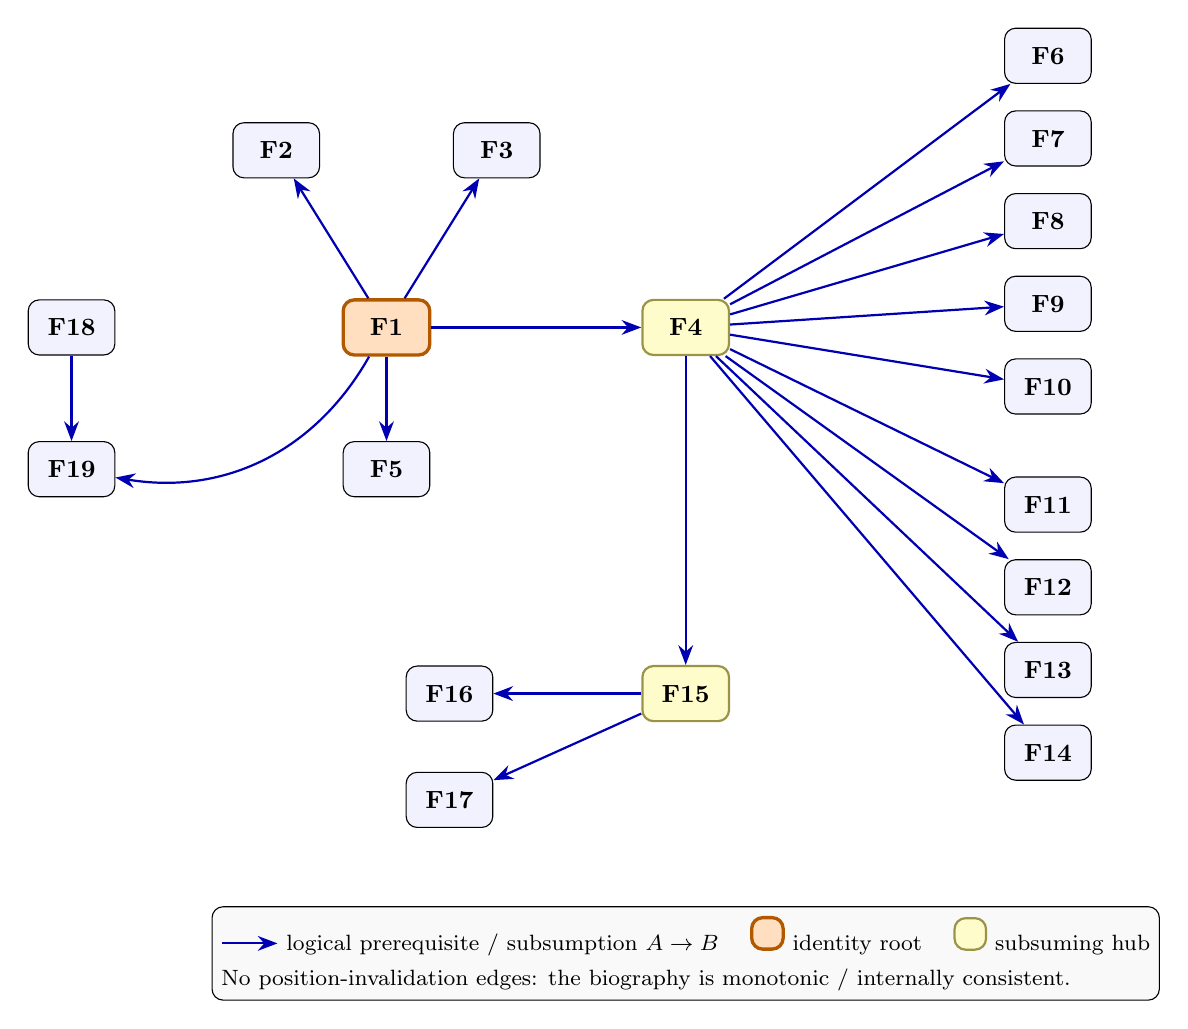
\begin{tikzpicture}[
    >={Stealth[length=2.5mm]},
    x=20mm, y=15mm,
    bnode/.style={draw,rounded corners,minimum width=11mm,minimum height=7mm,
                  inner sep=1pt,font=\small\bfseries,fill=blue!5},
    root/.style={bnode,fill=orange!25,draw=orange!70!black,very thick},
    hub/.style={bnode,fill=yellow!20,draw=yellow!55!black,thick},
    prereq/.style={->,blue!70!black,thick},
  ]

  % Explicit grid; generous spacing keeps every node clear of its neighbours
  % and of the edges. Films and TV are split into two separate columns so the
  % F4 fan-out never crowds a single tall stack.

  % --- persona (far left) ---
  \node[bnode] (f18) at (-2.0,1.7) {F18};
  \node[bnode] (f19) at (-2.0,0.5) {F19};

  % --- biographical facts (top, above the root) ---
  \node[bnode] (f2) at (-0.7,3.2) {F2};
  \node[bnode] (f3) at (0.7,3.2)  {F3};

  % --- root identity ---
  \node[root]  (f1) at (0,1.7) {F1};
  \node[bnode] (f5) at (0,0.5) {F5};

  % --- central "body of work" hub ---
  \node[hub] (f4) at (1.9,1.7) {F4};

  % --- film credits (right column, fanned upward) ---
  \node[bnode] (f6)  at (4.2,4.0) {F6};
  \node[bnode] (f7)  at (4.2,3.3) {F7};
  \node[bnode] (f8)  at (4.2,2.6) {F8};
  \node[bnode] (f9)  at (4.2,1.9) {F9};
  \node[bnode] (f10) at (4.2,1.2) {F10};

  % --- TV credits (right column, fanned downward; same column as films but
  %     a clear vertical gap below F10 so the fan never crosses a film node) ---
  \node[bnode] (f11) at (4.2,0.2)  {F11};
  \node[bnode] (f12) at (4.2,-0.5) {F12};
  \node[bnode] (f13) at (4.2,-1.2) {F13};
  \node[bnode] (f14) at (4.2,-1.9) {F14};

  % --- theater (below the hub, own column to the left of the credits) ---
  \node[hub]   (f15) at (1.9,-1.4) {F15};
  \node[bnode] (f16) at (0.4,-1.4) {F16};
  \node[bnode] (f17) at (0.4,-2.3) {F17};

  % --- edges from identity ---
  \draw[prereq] (f1) -- (f2);
  \draw[prereq] (f1) -- (f3);
  \draw[prereq] (f1) -- (f4);
  \draw[prereq] (f1) -- (f5);
  \draw[prereq] (f1) to[bend left=35] (f19);   % routed out to the left, clear of F18

  % --- F4 subsumes specific film credits ---
  \foreach \t in {f6,f7,f8,f9,f10} { \draw[prereq] (f4) -- (\t); }

  % --- F4 subsumes specific TV credits ---
  \foreach \t in {f11,f12,f13,f14} { \draw[prereq] (f4) -- (\t); }

  % --- F4 subsumes theater work, which subsumes the venues ---
  \draw[prereq] (f4) -- (f15);
  \draw[prereq] (f15) -- (f16);
  \draw[prereq] (f15) -- (f17);

  % --- persona cause ---
  \draw[prereq] (f18) -- (f19);

  % --- legend ---
  \node[draw,fill=gray!5,rounded corners,anchor=north,align=left,
        font=\footnotesize] at (1.9,-3.2) {
    \tikz\draw[prereq](0,0)--(7mm,0);~logical prerequisite / subsumption $A\rightarrow B$
    \quad
    \tikz\node[root,minimum width=4mm,minimum height=4mm]{};~identity root
    \quad
    \tikz\node[hub,minimum width=4mm,minimum height=4mm]{};~subsuming hub\\[3pt]
    No position-invalidation edges: the biography is monotonic / internally consistent.
  };

\end{tikzpicture}
\end{center}

\subsection*{A modified biography with planted contradictions}

The biography above is internally consistent, so it has no invalidation edges.
To illustrate the contradiction relation we now \emph{alter} the passage,
inserting later statements that conflict with earlier ones (different birth year
and place, a different nationality, a different career-start decade, and a voice
description that reverses the earlier one). Each contradiction is a positional
invalidation: the earlier atom, asserted first, is contradicted by a later atom.

\paragraph{Modified source paragraph (contradictions in \emph{italics}).}

\noindent\textbf{Plain text.}
\begin{quote}
Lanny Flaherty is an American actor born on December 18, 1949, in Pensacola,
Florida. His career began in the late 1970s, and he appeared in numerous films,
television shows, and theater productions. He is known for his deep gravelly
voice. \emph{Born in 1942, Flaherty was a Mississippi native who first appeared
on screen only in the 1990s.} Critics often described \emph{the British
character actor} for \emph{his soft, high-pitched voice}, which made him
instantly recognizable.
\end{quote}

\noindent\textbf{Annotated.} Each clause is one atomic unit
\textsuperscript{\textbf{\scriptsize M\textit{n}}}. Green marks an
earlier (asserted-first) atom and red the later atom that contradicts it; neutral
(blue) atoms are uncontested.

\begin{quote}
\fu{cEarly}{Lanny Flaherty is an American actor}{M1} born
\fu{cEarly}{on December 18, 1949}{M2}, \fu{cEarly}{in Pensacola, Florida}{M3}.
\fu{cEarly}{His career began in the late 1970s}{M4}, and
\fu{cId}{he appeared in numerous films, television shows, and theater productions}{M5}.
\fu{cEarly}{He is known for his deep gravelly voice}{M6}.
\emph{\fu{cLate}{Born in 1942}{M7}, \fu{cLate}{Flaherty was a Mississippi native}{M8}
\fu{cLate}{who first appeared on screen only in the 1990s}{M9}.} Critics often
described \emph{\fu{cLate}{the British character actor}{M10}} for
\emph{\fu{cLate}{his soft, high-pitched voice}{M11}}, which
\fu{cId}{made him instantly recognizable}{M12}.
\end{quote}

\paragraph{Atomic units (self-contained, in order of appearance).}
\begin{enumerate}[label=\textbf{M\arabic*.},leftmargin=*]
  \item Lanny Flaherty is an American actor.
  \item Lanny Flaherty was born on December 18, 1949.
  \item Lanny Flaherty was born in Pensacola, Florida.
  \item Lanny Flaherty's career began in the late 1970s.
  \item Lanny Flaherty appeared in numerous films, television shows, and theater productions.
  \item Lanny Flaherty is known for his deep gravelly voice.
  \item Lanny Flaherty was born in 1942.
  \item Lanny Flaherty was a Mississippi native.
  \item Lanny Flaherty first appeared on screen only in the 1990s.
  \item Lanny Flaherty is a British character actor.
  \item Lanny Flaherty has a soft, high-pitched voice.
  \item Lanny Flaherty's voice made him instantly recognizable.
\end{enumerate}

\subsubsection*{Relations}

\textbf{Logical prerequisites ($A \rightarrow B$).}
\begin{itemize}[leftmargin=*]
  \item M1 $\rightarrow$ M5 --- being an actor is presupposed by having a body of acting work.
  \item M1 $\rightarrow$ M4 --- being an actor is presupposed by having an acting career.
  \item M11 $\rightarrow$ M12 --- having a (distinctive) voice is presupposed by that voice making him recognizable.
\end{itemize}

\noindent
\textbf{Position invalidations ($A \neq B$).} Each later atom contradicts an
earlier one asserted at a different position.
\begin{itemize}[leftmargin=*]
  \item M2 $\neq$ M7 --- born December 18, 1949 contradicts born in 1942.
  \item M3 $\neq$ M8 --- born in Pensacola, Florida contradicts being a Mississippi native.
  \item M4 $\neq$ M9 --- a career beginning in the late 1970s contradicts first appearing on screen only in the 1990s.
  \item M1 $\neq$ M10 --- being an \emph{American} actor contradicts being a \emph{British} character actor.
  \item M6 $\neq$ M11 --- a deep gravelly voice contradicts a soft, high-pitched voice.
\end{itemize}

\noindent
\textbf{Note.} The contradictions are pairwise and local: each invalidation links
exactly one early biographical claim to its later mutually exclusive restatement.
The prerequisite structure (identity $\to$ work / career, voice $\to$
recognizability) is unaffected; M5 has no specific-credit children here because
the modified paragraph drops the individual titles.

\paragraph{Relation graph.}
Solid blue arrows are logical prerequisites ($A \rightarrow B$). Dashed red
arrows are position invalidations ($A \neq B$): each links an earlier
(\emph{green, asserted-first}) atom to the later (\emph{red}) atom that
contradicts it. The five contradiction pairs are stacked so no arrow crosses a
node.

\begin{center}
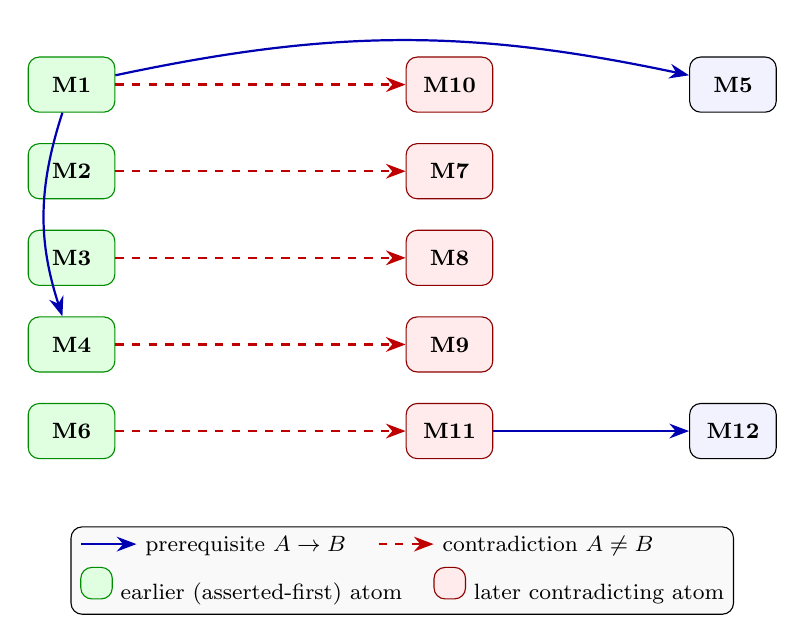
\begin{tikzpicture}[
    >={Stealth[length=2.5mm]},
    x=20mm, y=11mm,
    mnode/.style={draw,rounded corners,minimum width=11mm,minimum height=7mm,
                  inner sep=1pt,font=\footnotesize\bfseries,fill=blue!5},
    early/.style={mnode,fill=green!12,draw=green!55!black},
    late/.style={mnode,fill=red!8,draw=red!55!black},
    prereq/.style={->,blue!70!black,thick},
    invalid/.style={->,red!75!black,dashed,thick},
  ]

  % Left column: earlier (asserted-first) atoms. Right column: the later atoms
  % that contradict them. Each contradiction pair sits on its own row, so the
  % dashed edges are short horizontals that never cross a node.
  \node[early] (m1) at (0,4) {M1};
  \node[early] (m2) at (0,3) {M2};
  \node[early] (m3) at (0,2) {M3};
  \node[early] (m4) at (0,1) {M4};
  \node[early] (m6) at (0,0) {M6};

  \node[late] (m10) at (2.4,4) {M10};
  \node[late] (m7)  at (2.4,3) {M7};
  \node[late] (m8)  at (2.4,2) {M8};
  \node[late] (m9)  at (2.4,1) {M9};
  \node[late] (m11) at (2.4,0) {M11};

  % prerequisite-only atoms (right side, kept clear of the contradiction fan)
  \node[mnode] (m5)  at (4.2,4) {M5};
  \node[mnode] (m12) at (4.2,0) {M12};

  % --- contradiction edges (one per row) ---
  \draw[invalid] (m1) -- (m10);
  \draw[invalid] (m2) -- (m7);
  \draw[invalid] (m3) -- (m8);
  \draw[invalid] (m4) -- (m9);
  \draw[invalid] (m6) -- (m11);

  % --- prerequisite edges ---
  \draw[prereq] (m1) to[bend left=12] (m5);   % identity -> body of work
  \draw[prereq] (m1) to[bend right=18] (m4);   % identity -> career
  \draw[prereq] (m11) -- (m12);                % voice -> recognizable

  % --- legend ---
  \node[draw,fill=gray!5,rounded corners,anchor=north,align=left,
        font=\footnotesize] at (2.1,-1.1) {
    \tikz\draw[prereq](0,0)--(7mm,0);~prerequisite $A\rightarrow B$
    \quad
    \tikz\draw[invalid](0,0)--(7mm,0);~contradiction $A\neq B$\\[3pt]
    \tikz\node[early,minimum width=4mm,minimum height=4mm]{};~earlier (asserted-first) atom
    \quad
    \tikz\node[late,minimum width=4mm,minimum height=4mm]{};~later contradicting atom
  };

\end{tikzpicture}
\end{center}

\end{document}
